
    \documentclass{article}

    %  Русский язык

    \usepackage[T2A]{fontenc}			% кодировка
    \usepackage[utf8]{inputenc}			% кодировка исходного текста
    \usepackage[english,russian]{babel}	% локализация и переносы
    \usepackage{unicode-math}

    % Рисунки
    \usepackage{graphicx, float}
    \usepackage{wrapfig}


    \title{Wild wild west derivative counter}
    \author{Dodo}
    \date{November 2022}


    \begin{document}
    \maketitle
    
        Welcome to derivative calculator fella, let's have a look at ya. God, what da hell is dis shit, fella?
        Ok, ok, let's calculate this bullshit.

        \begin{center}\begin{center} 
\includegraphics[scale=0.6]{funny_pics/cowboy.jpg} \end{center}\end{center}
        \begin{center}
        $\clubsuit$~$\clubsuit$~$\clubsuit$
        \end{center}

    \begin{center} 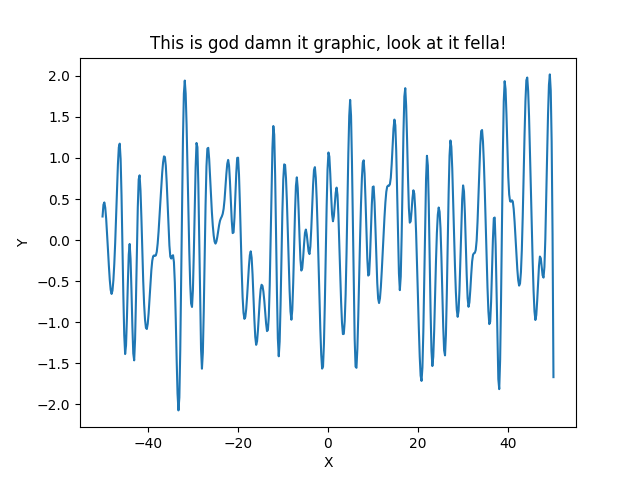
\includegraphics[scale=0.6]{function_graph.png} \end{center}Alright fella, let's look wat we got, i haven't seen so beautiful trees for ages:
\begin{center} 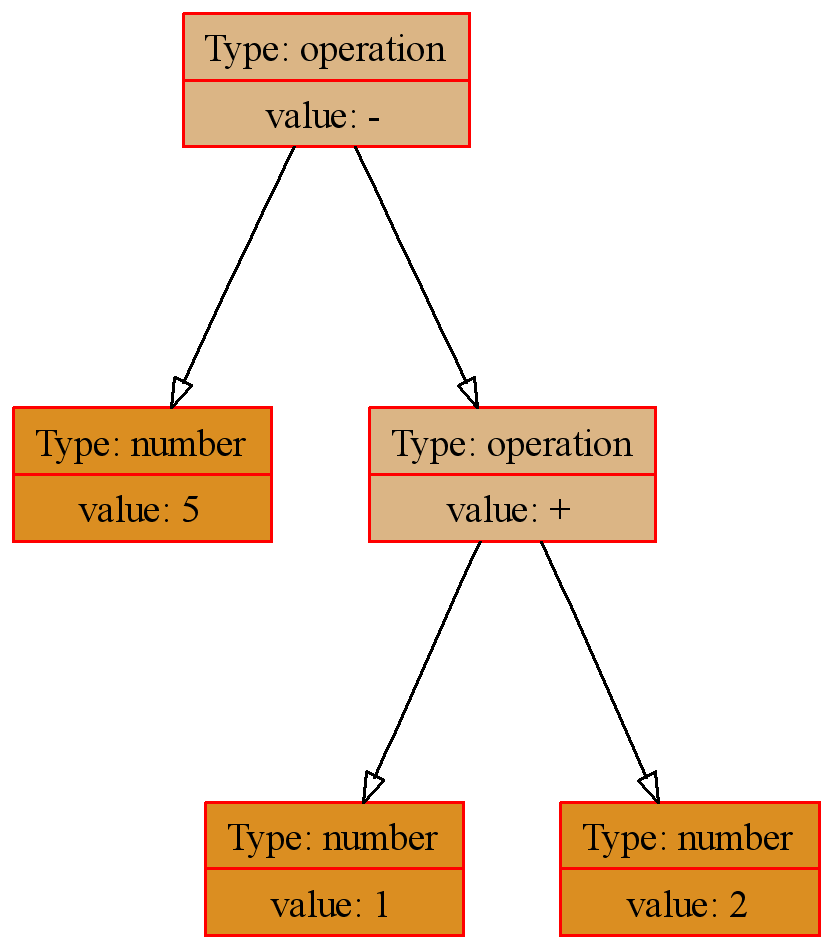
\includegraphics[scale=0.2]{pretty_tree0.png} \end{center}
\begin{center}$
{{sin{({{X}^{5}})}}+{{({cos{({{10}\cdot{X}})}})}^{({3})}}}
$\end{center}
\begin{center} $\clubsuit$~$\clubsuit$~$\clubsuit$ \end{center}\begin{center}  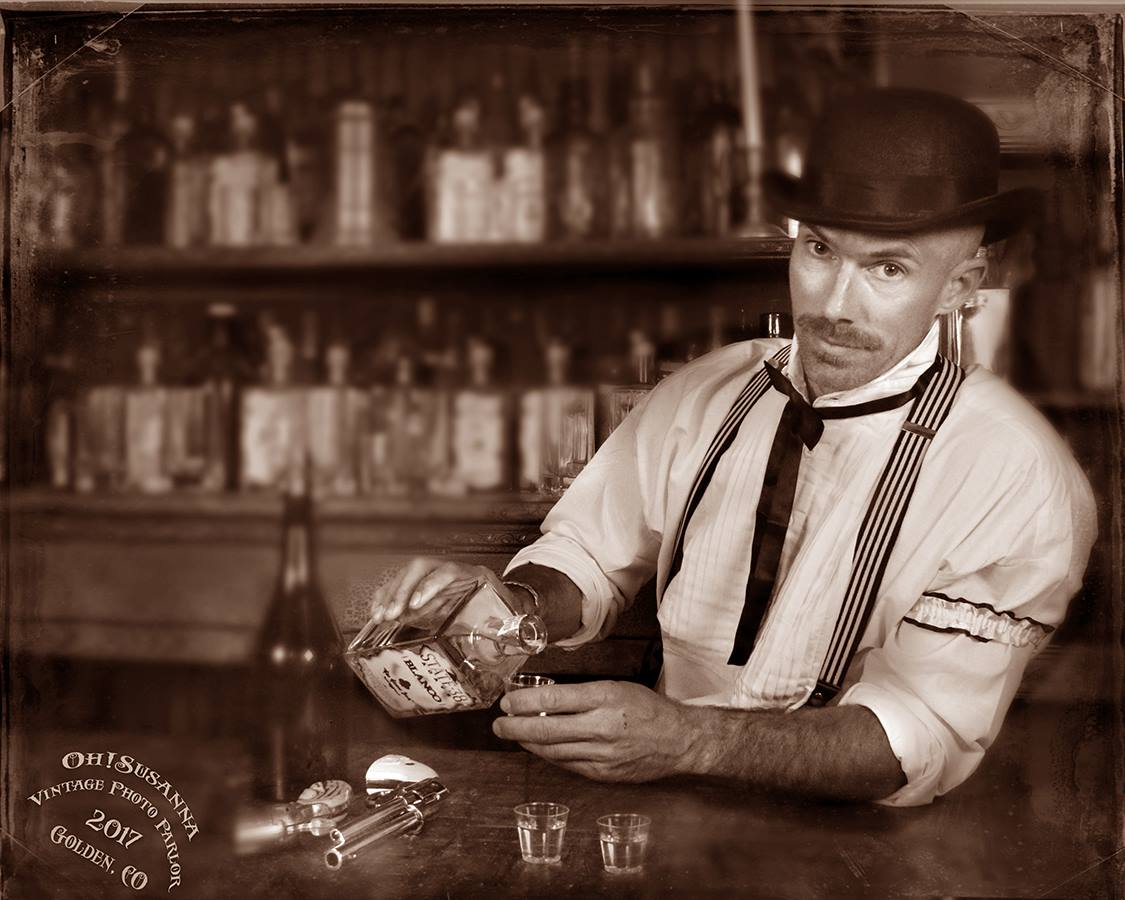
\includegraphics[scale=0.3]{funny_pics/bartender.jpg} \end{center} With the power of gods, let's write the following: 
\begin{center}$
{{{0}\cdot{X}}+{{10}\cdot{1}}}
$\end{center}
\begin{center} $\clubsuit$~$\clubsuit$~$\clubsuit$ \end{center}\begin{center}  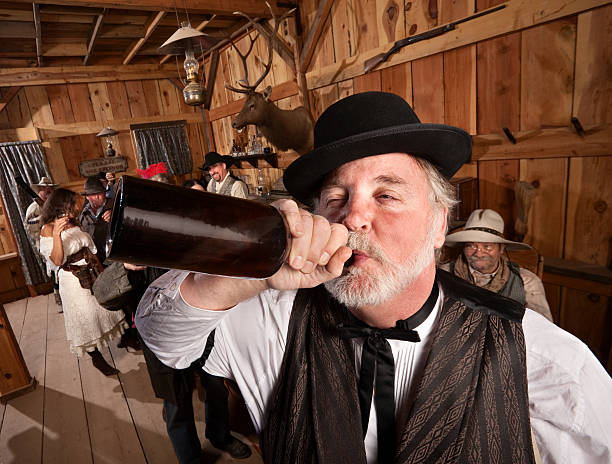
\includegraphics[scale=1.4]{funny_pics/drunk_cowboy.jpg} \end{center} I smacked a damn big cockroach yesterday fella, this was left on my shoe: 
\begin{center}$
{{({{({-1})}\cdot{({sin{({{10}\cdot{X}})}})}})}\cdot{({10})}}
$\end{center}
\begin{center} $\clubsuit$~$\clubsuit$~$\clubsuit$ \end{center}\begin{center} 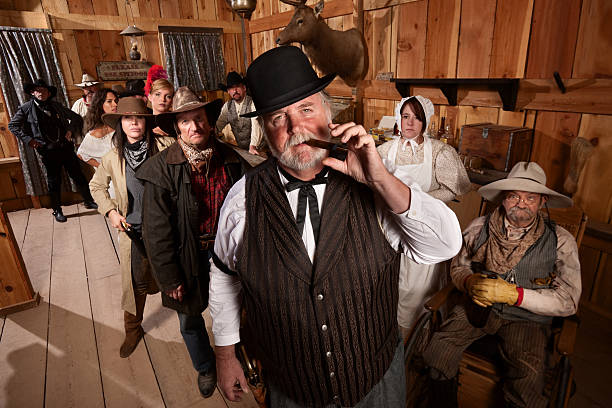
\includegraphics[scale=1.4]{funny_pics/funny_bartender.jpg} \end{center} Don't distract fella, I don't know how to count
\begin{center}$
{{({{({3})}\cdot{({{({cos{({{10}\cdot{X}})}})}^{({2})}})}})}\cdot{({{({{({-1})}\cdot{({sin{({{10}\cdot{X}})}})}})}\cdot{({10})}})}}
$\end{center}
\begin{center} $\clubsuit$~$\clubsuit$~$\clubsuit$ \end{center}\begin{center}  
\includegraphics[scale=0.3]{funny_pics/cowboy_cat.jpg} \end{center}Oh come on, my wife is pregnant 12th time in a row.
\begin{center}$
{{({{({5})}\cdot{({{X}^{4}})}})}\cdot{({1})}}
$\end{center}
\begin{center} $\clubsuit$~$\clubsuit$~$\clubsuit$ \end{center}\begin{center}  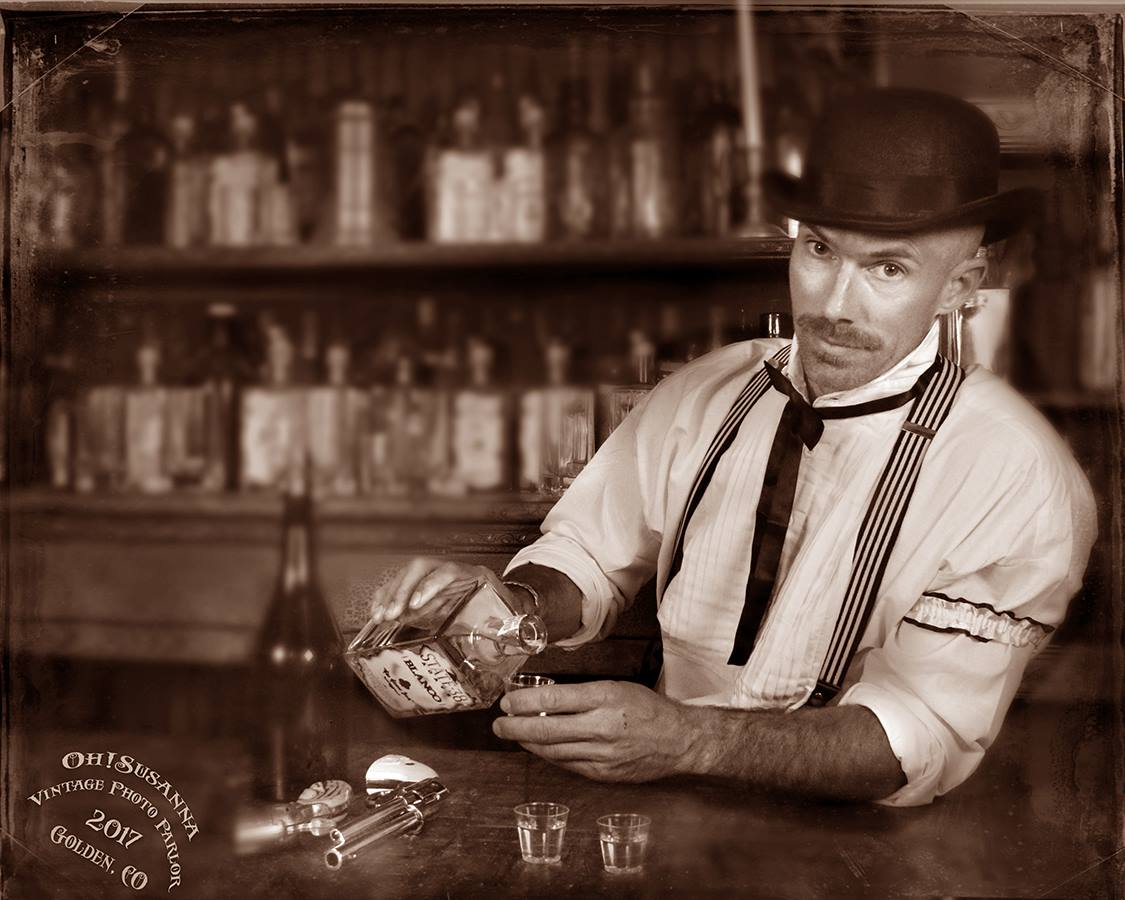
\includegraphics[scale=0.3]{funny_pics/bartender.jpg} \end{center}Can you understand it by yourself, i must go get some beer, fella:
\begin{center}$
{{({cos{({{X}^{5}})}})}\cdot{({{({{({5})}\cdot{({{X}^{4}})}})}\cdot{({1})}})}}
$\end{center}
\begin{center} $\clubsuit$~$\clubsuit$~$\clubsuit$ \end{center}...
\begin{center}$
{{{({cos{({{X}^{5}})}})}\cdot{({{({{({5})}\cdot{({{X}^{4}})}})}\cdot{({1})}})}}+{{({{({3})}\cdot{({{({cos{({{10}\cdot{X}})}})}^{({2})}})}})}\cdot{({{({{({-1})}\cdot{({sin{({{10}\cdot{X}})}})}})}\cdot{({10})}})}}}
$\end{center}
\begin{center} $\clubsuit$~$\clubsuit$~$\clubsuit$ \end{center}Here is whach you got, fella. Now let's drink some whiskey and shoot niggers.\begin{center} 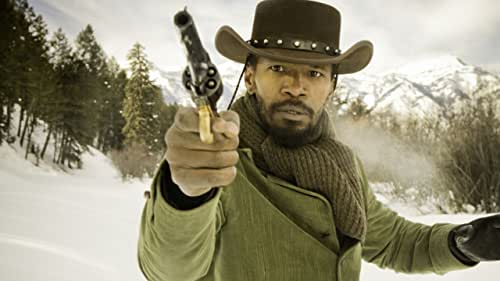
\includegraphics[scale=0.6]{funny_pics/slave.jpg} \end{center}
\begin{center}$
{{{({cos{({{X}^{5}})}})}\cdot{({{({{({5})}\cdot{({{X}^{4}})}})}\cdot{({1})}})}}+{{({{({3})}\cdot{({{({cos{({{10}\cdot{X}})}})}^{({2})}})}})}\cdot{({{({{({-1})}\cdot{({sin{({{10}\cdot{X}})}})}})}\cdot{({10})}})}}}
$\end{center}
\begin{center} $\clubsuit$~$\clubsuit$~$\clubsuit$ \end{center}Alright fella, let's make this shit called Macloren,there will be only 3 steps, cause i don't know how to count more.Basicly the main formula will look like that
 \[ f(x) = f(0) + \frac{f^{(1)}(0)}{1!}\cdot X + \frac{f^{(2)}(0)}{2!}\cdot X + \frac{f^{(3)}(0)}{3!}\cdot X + \text{...}\]
\[ f^{(0)}(0) = 1\]\[ f^{(1)}(0) = 0\]\[ f^{(2)}(0) = -300\]\[ f^{(3)}(0) = 0\]
        The solution is pretty simple and you definetely can do it \textbf{yourself}
        \end{document}
    